\section{Arquitectura}

El sistema adoptará una \textbf{arquitectura cliente-servidor} con un backend
monolítico modular, implementando el patrón de diseño \textit{gateway
aggregation} con el objetivo de centralizar la lógica de integración con
múltiples fuentes externas.

El patrón gateway aggregation —mostrado en la
Figura~\ref{fig:gateway-aggregation}— consiste en utilizar un componente
intermediario que recibe una sola petición del cliente, la descompone en
múltiples llamadas a servicios backend, agrega los resultados y devuelve una
única respuesta.


\begin{figure}[h!]
    \centering
    \fbox{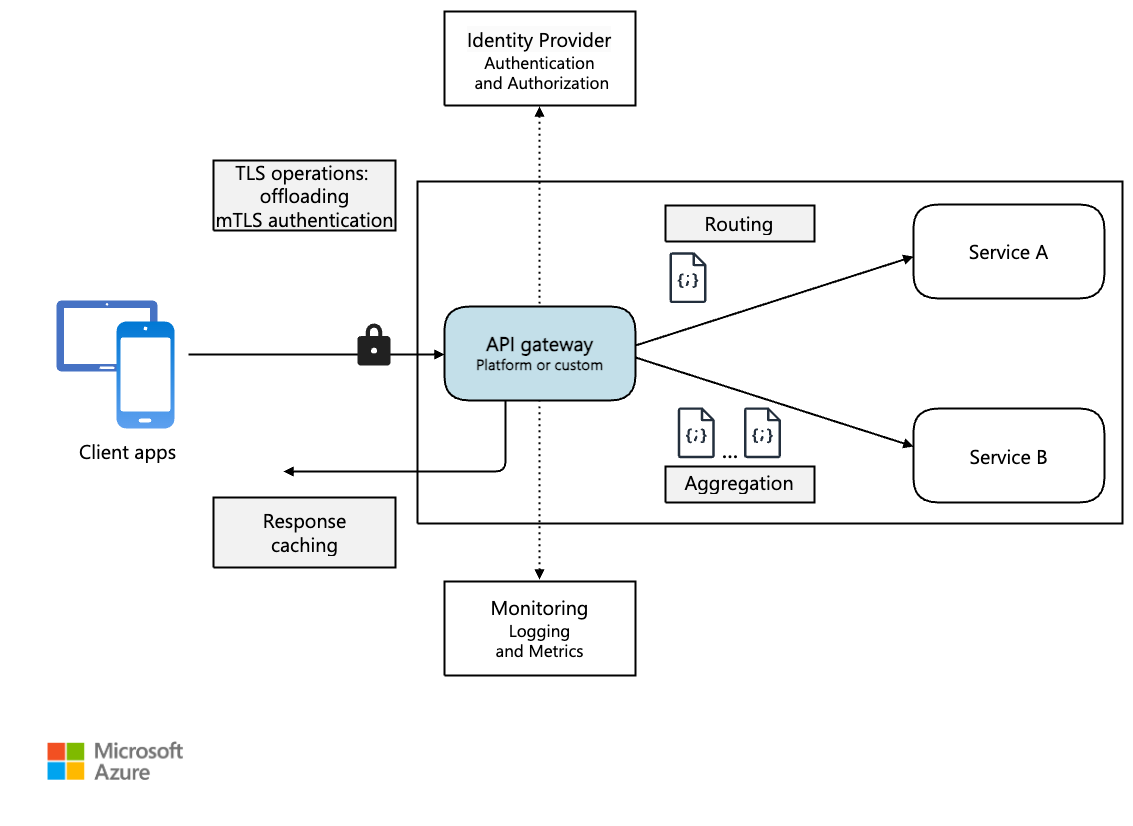
\includegraphics[width=0.8\textwidth]{imagenes/gateway-aggregation.png}}
    \caption{Gateway Aggregation}\label{fig:gateway-aggregation}
\end{figure}

\begin{figure}[h!]
    \centering
    \fbox{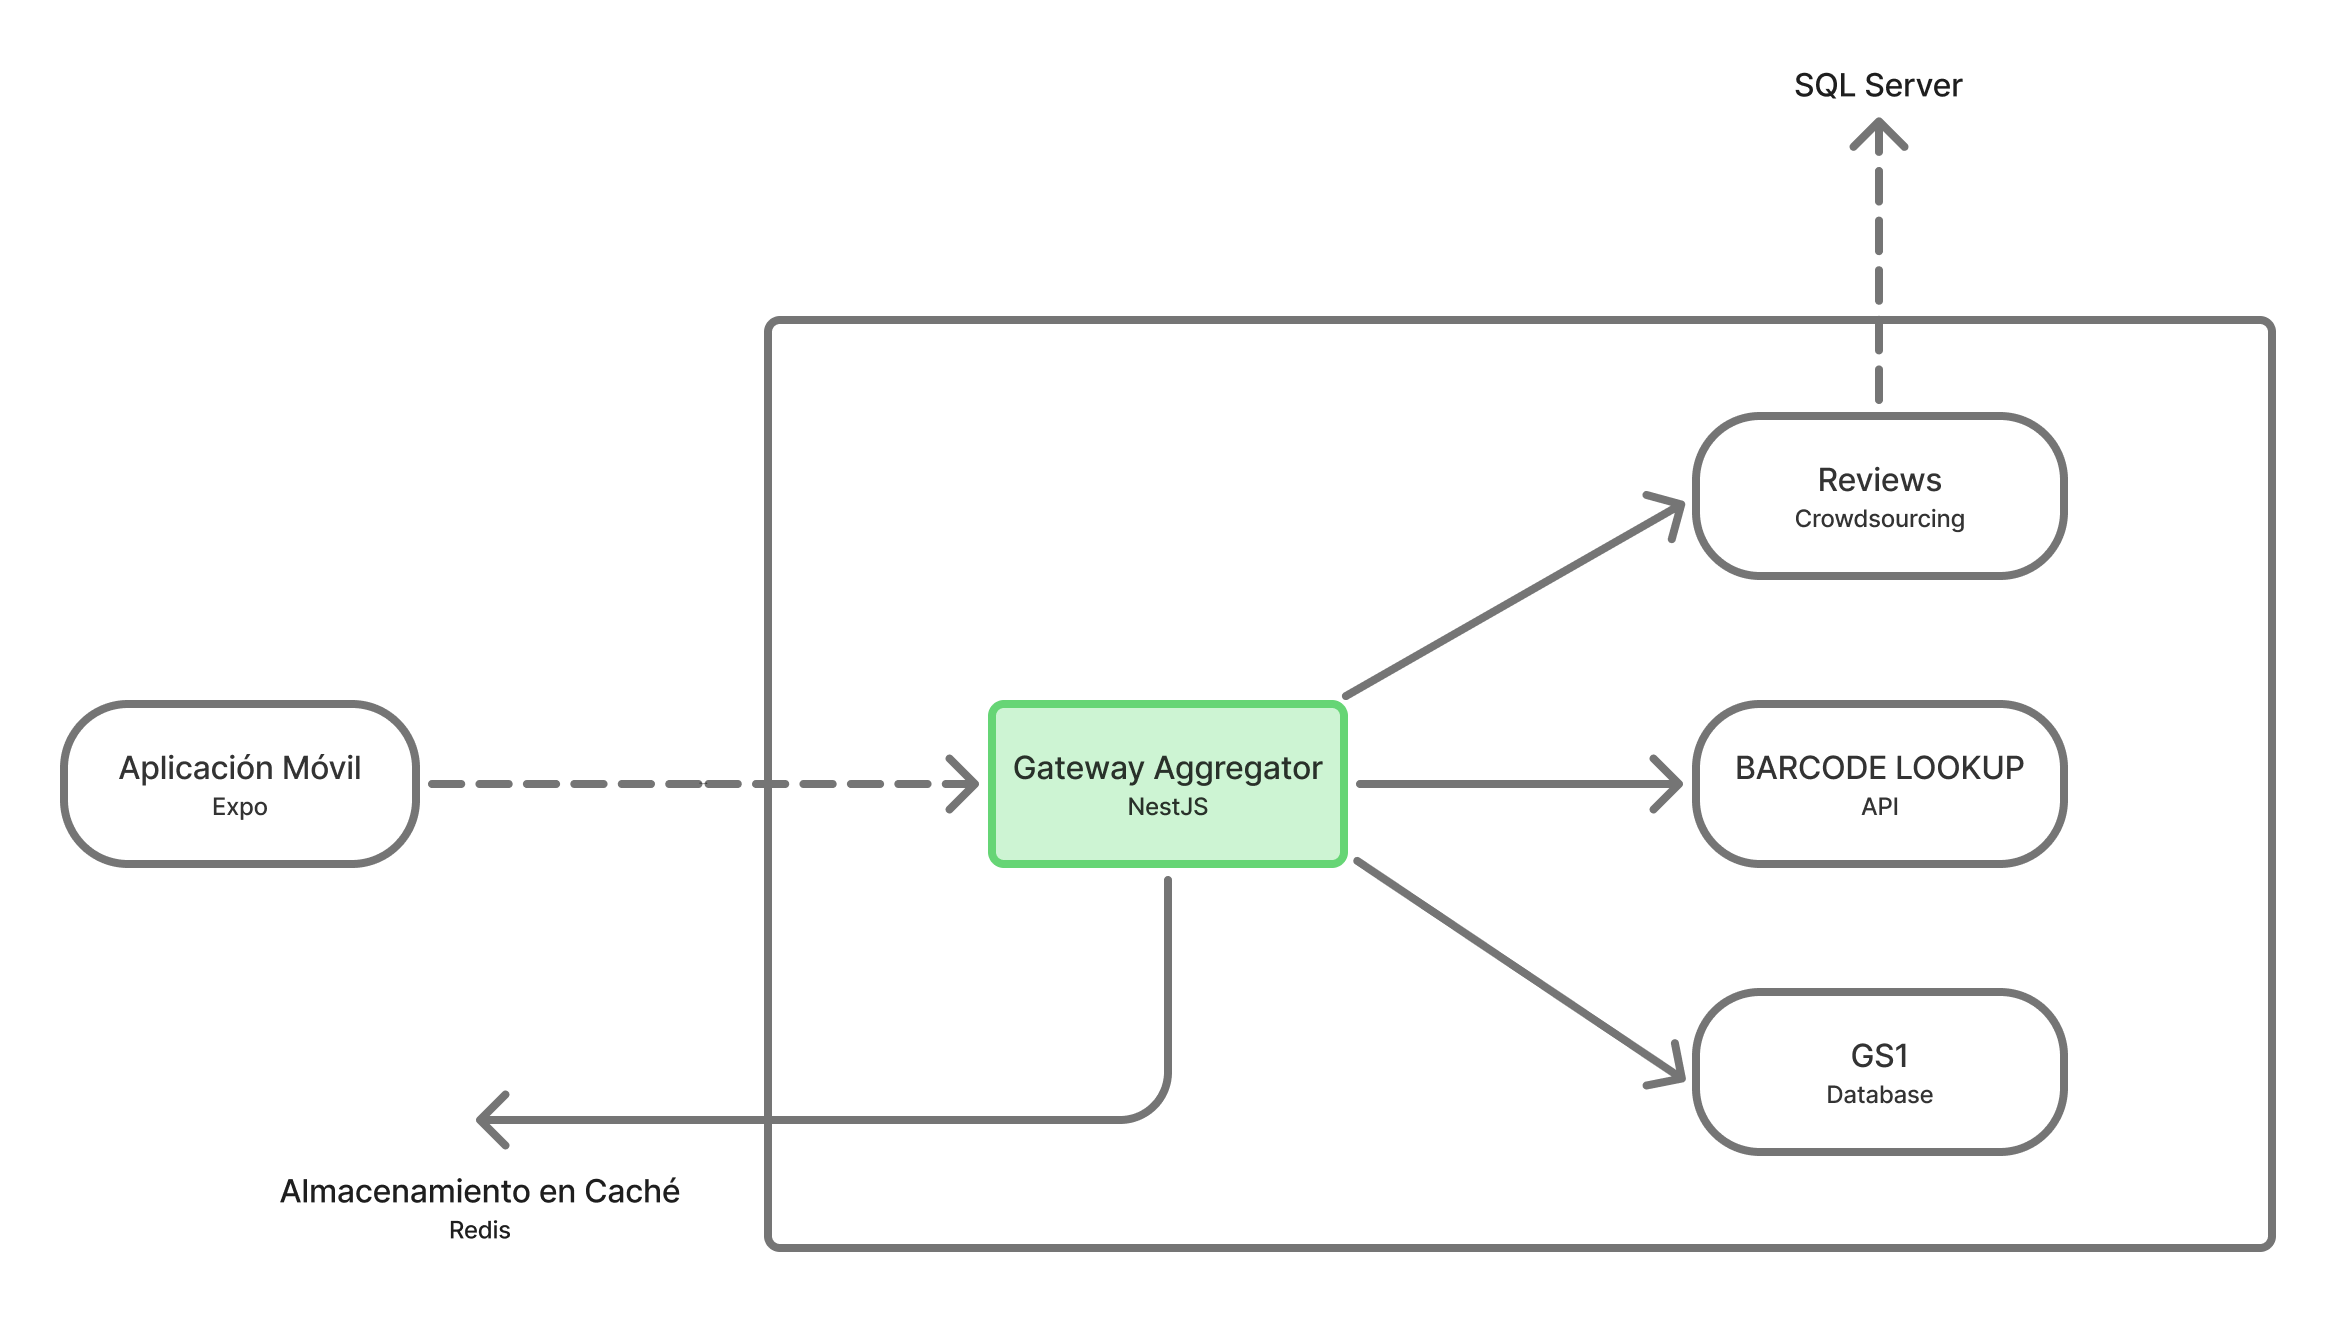
\includegraphics[width=0.8\textwidth]{imagenes/diagrama-sistema.png}}
    \caption{Diagrama del Sistema}\label{fig:diagrama-sistema}
\end{figure}